\section{Pre-Trained Models}
This section describes the results obtained using different pre-trained architecture and strategies. The pre-trained networks here tested are:
\begin{itemize}
\item VGG16
\item ResNet50V2
\item ResNet101V2
\item InceptionV3
\end{itemize}

 
 
\subsection{VGG16}

\subsubsection{Test 1: Classical VGG16 (Feature Extraction)}
VGG16\ref{fig:vgg16} is a convolutional neural network model proposed by Simonyan et al., with several 3x3 convolutional layers in cascade occasionally interleaved with 2x2 max-pooling layers forming the so called \textit{blocks}. Developed for the ILSVRC2014 challenge, it was able to achieve a top-5 accuracy of 92.7 on ImageNet.
\begin{figure}[H]
	\centering
	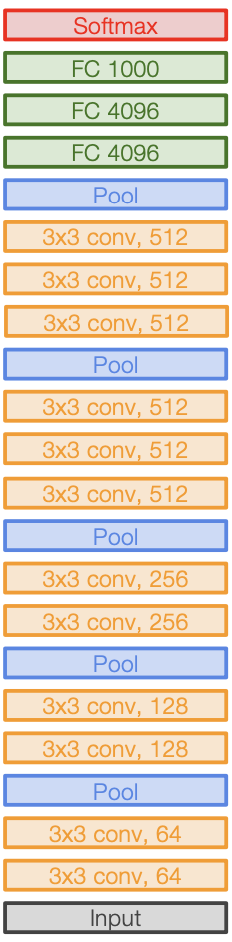
\includegraphics[height=0.3\textwidth]{img/vgg16.png}
	\caption{VGG16 Architecture}
	\label{fig:vgg16}
\end{figure}

\subsubsection{Test 2: Test 1 with Data Augmentation}


\subsubsection{Test 3: Completely New Output Layers Architecture (Feature Extraction)}

\subsubsection{Test 4: Test 4 with Data Augmentation}

\subsubsection{Test 5: Test 4 with Data Augmentation + Regularization}

\subsubsection{Test 6: Fine Tuning with One Layer}

\subsubsection{Test 7: Fine Tuning with Two Layers}

\subsubsection{Test 8: Genetic Algorithm for Hyper-parameters and Architecture Optimization}





\subsection{ResNet50V2}

\subsubsection{Test 1: Classical ResNet50V2 (Feature Extraction)}
On a small dataset, overfitting will be the main issue. Data augmentation is a powerful way to fight overfitting when you’re working with image data.

\subsubsection{Test 2: Completely New Output Layers Architecture}

\subsubsection{Test 3: 1 and 2 with Data Augmentation}

\subsubsection{Test 4: Fine Tuning with One Layer}

\subsubsection{Test 5: Fine Tuning with Two Layers}







\subsection{ResNet101V2}

\subsubsection{Test 1: Classical ResNet101V2 with 50 classes}

\subsubsection{Test 2: Completely Newly Output Layers Architecture}

\subsubsection{Test 3: Fine Tuning with One Layer}

\subsubsection{Test 4: Fine Tuning with Two Layers}







\subsection{InceptionV3}

\subsubsection{Test 1: Classical ResNet101V2 with 50 classes}

\subsubsection{Test 2: Completely Newly Output Layers Architecture}

\subsubsection{Test 3: Fine Tuning with One Layer}

\subsubsection{Test 4: Fine Tuning with Two Layers}
